\documentclass[a4paper,13pt]{article}
\usepackage[MeX]{polski}
\usepackage[hidelinks]{hyperref}
\usepackage{color}
\usepackage{mathtools}
\usepackage{float}
\usepackage[OT4]{fontenc}
\usepackage{listings}
\usepackage[margin=1in]{geometry}

\frenchspacing




\lstset{
	language=C++,
	breaklines=true,
	postbreak=\mbox{\textcolor{red}{$\hookrightarrow$}\space},
	literate={ą}{{\,a}}1 {ę}{{\,e}}1 {ó}{{\'o}}1 {ż}{{\*z}}1 {ź}{{\'z}}1 {ł}{{\'l}}1 {ś}{{\'s}}1 {ć}{{\'c}}1 {ń}{{\'n}}1
}


\title{Projekt robota trójnożnego}
\author{Jakub Mazur}
\date{\today}


\begin{document}

%\begin{lstlisting}
%ą ę ż ł
%\end{lstlisting}
% TODO - ogarnąć encoding


\maketitle

\hypersetup{
	linktocpage=true,
    colorlinks=true,
    urlcolor=red,
    linktoc=all,
    linkcolor=blue,
}
\tableofcontents

\section{Model Matematyczny}
Noga ma 3 stopnie swobody. Wszystkie są typu obrotowego, przy czym dwie obracają się dookoła osi poziomej, a jedna dookoła osi pionowej. Są to te same osi obrotu co w przypadku ramienia robotycznego typu antromorficznego.
\subsection{Noga robota typu RRR}
Jest to noga o 3 rotacyjnych stopniach swobody, przy czym 1 stopień obraca się dookoła osi z, a 2 stopnie dookoła osi y. Model matematyczny takiej nogi, a co za tym idzie także jej kinematyka, będzie identyczny jak model ramienia robotycznego typu antropomorficznego (zwanego także "angular" bądź "jointed").

\begin{figure}[H]
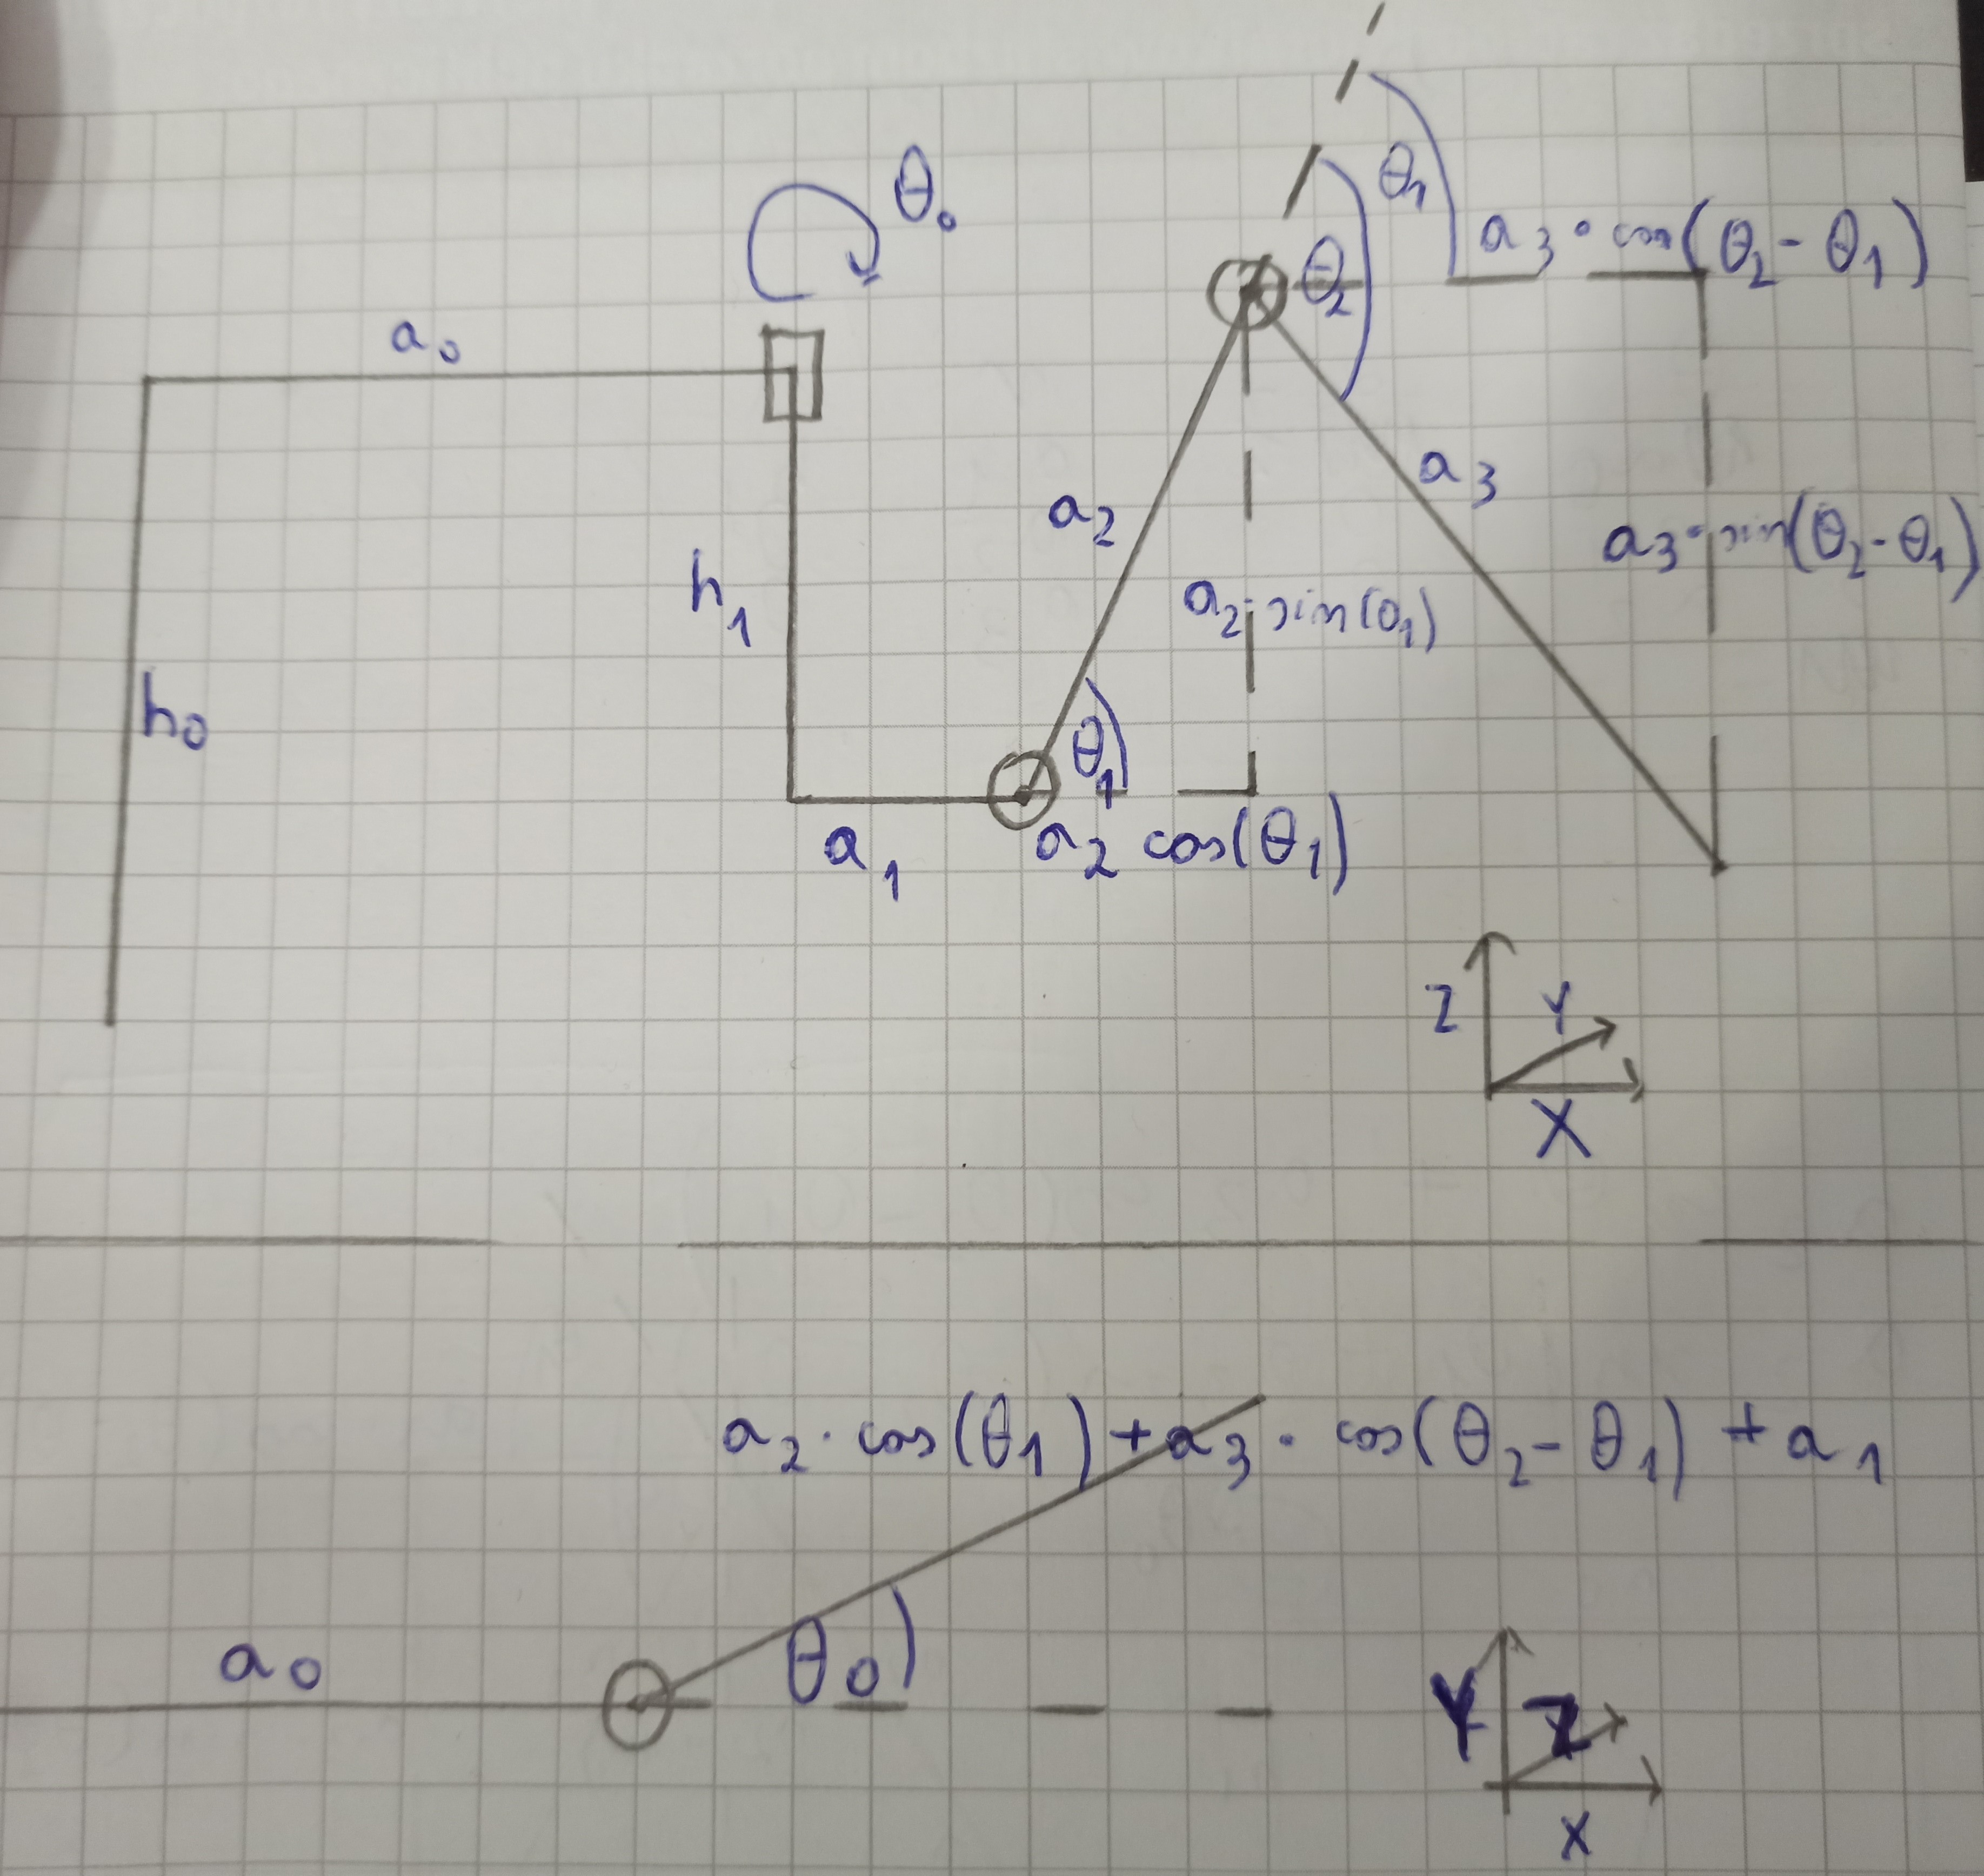
\includegraphics[width=\textwidth]{img/math_model.jpg}
\caption{Model Matematyczny}
\label{math_model}
\end{figure}

\subsubsection{Forward kinematics}

\begin{equation} \label{FK_ver_1}
\begin{split}
a_{temp} &= a_2 \cos{\theta_1} + a_3 \cos{\left(\theta_2 - \theta_1\right)} + a_1\\
Y &= a_{temp} \cdot \sin{\theta_0}\\
X &= a_{temp} \cdot \cos{\theta_0}\\
Z &= a_2 \sin{\theta_1} - a_3 \sin{\left(\theta_2 - \theta_1\right)}
\end{split}
\end{equation}

\subsubsection{Forward kinematics - denavit hartenberg \cite{DH_AA_article}}

\begin{figure}[H]
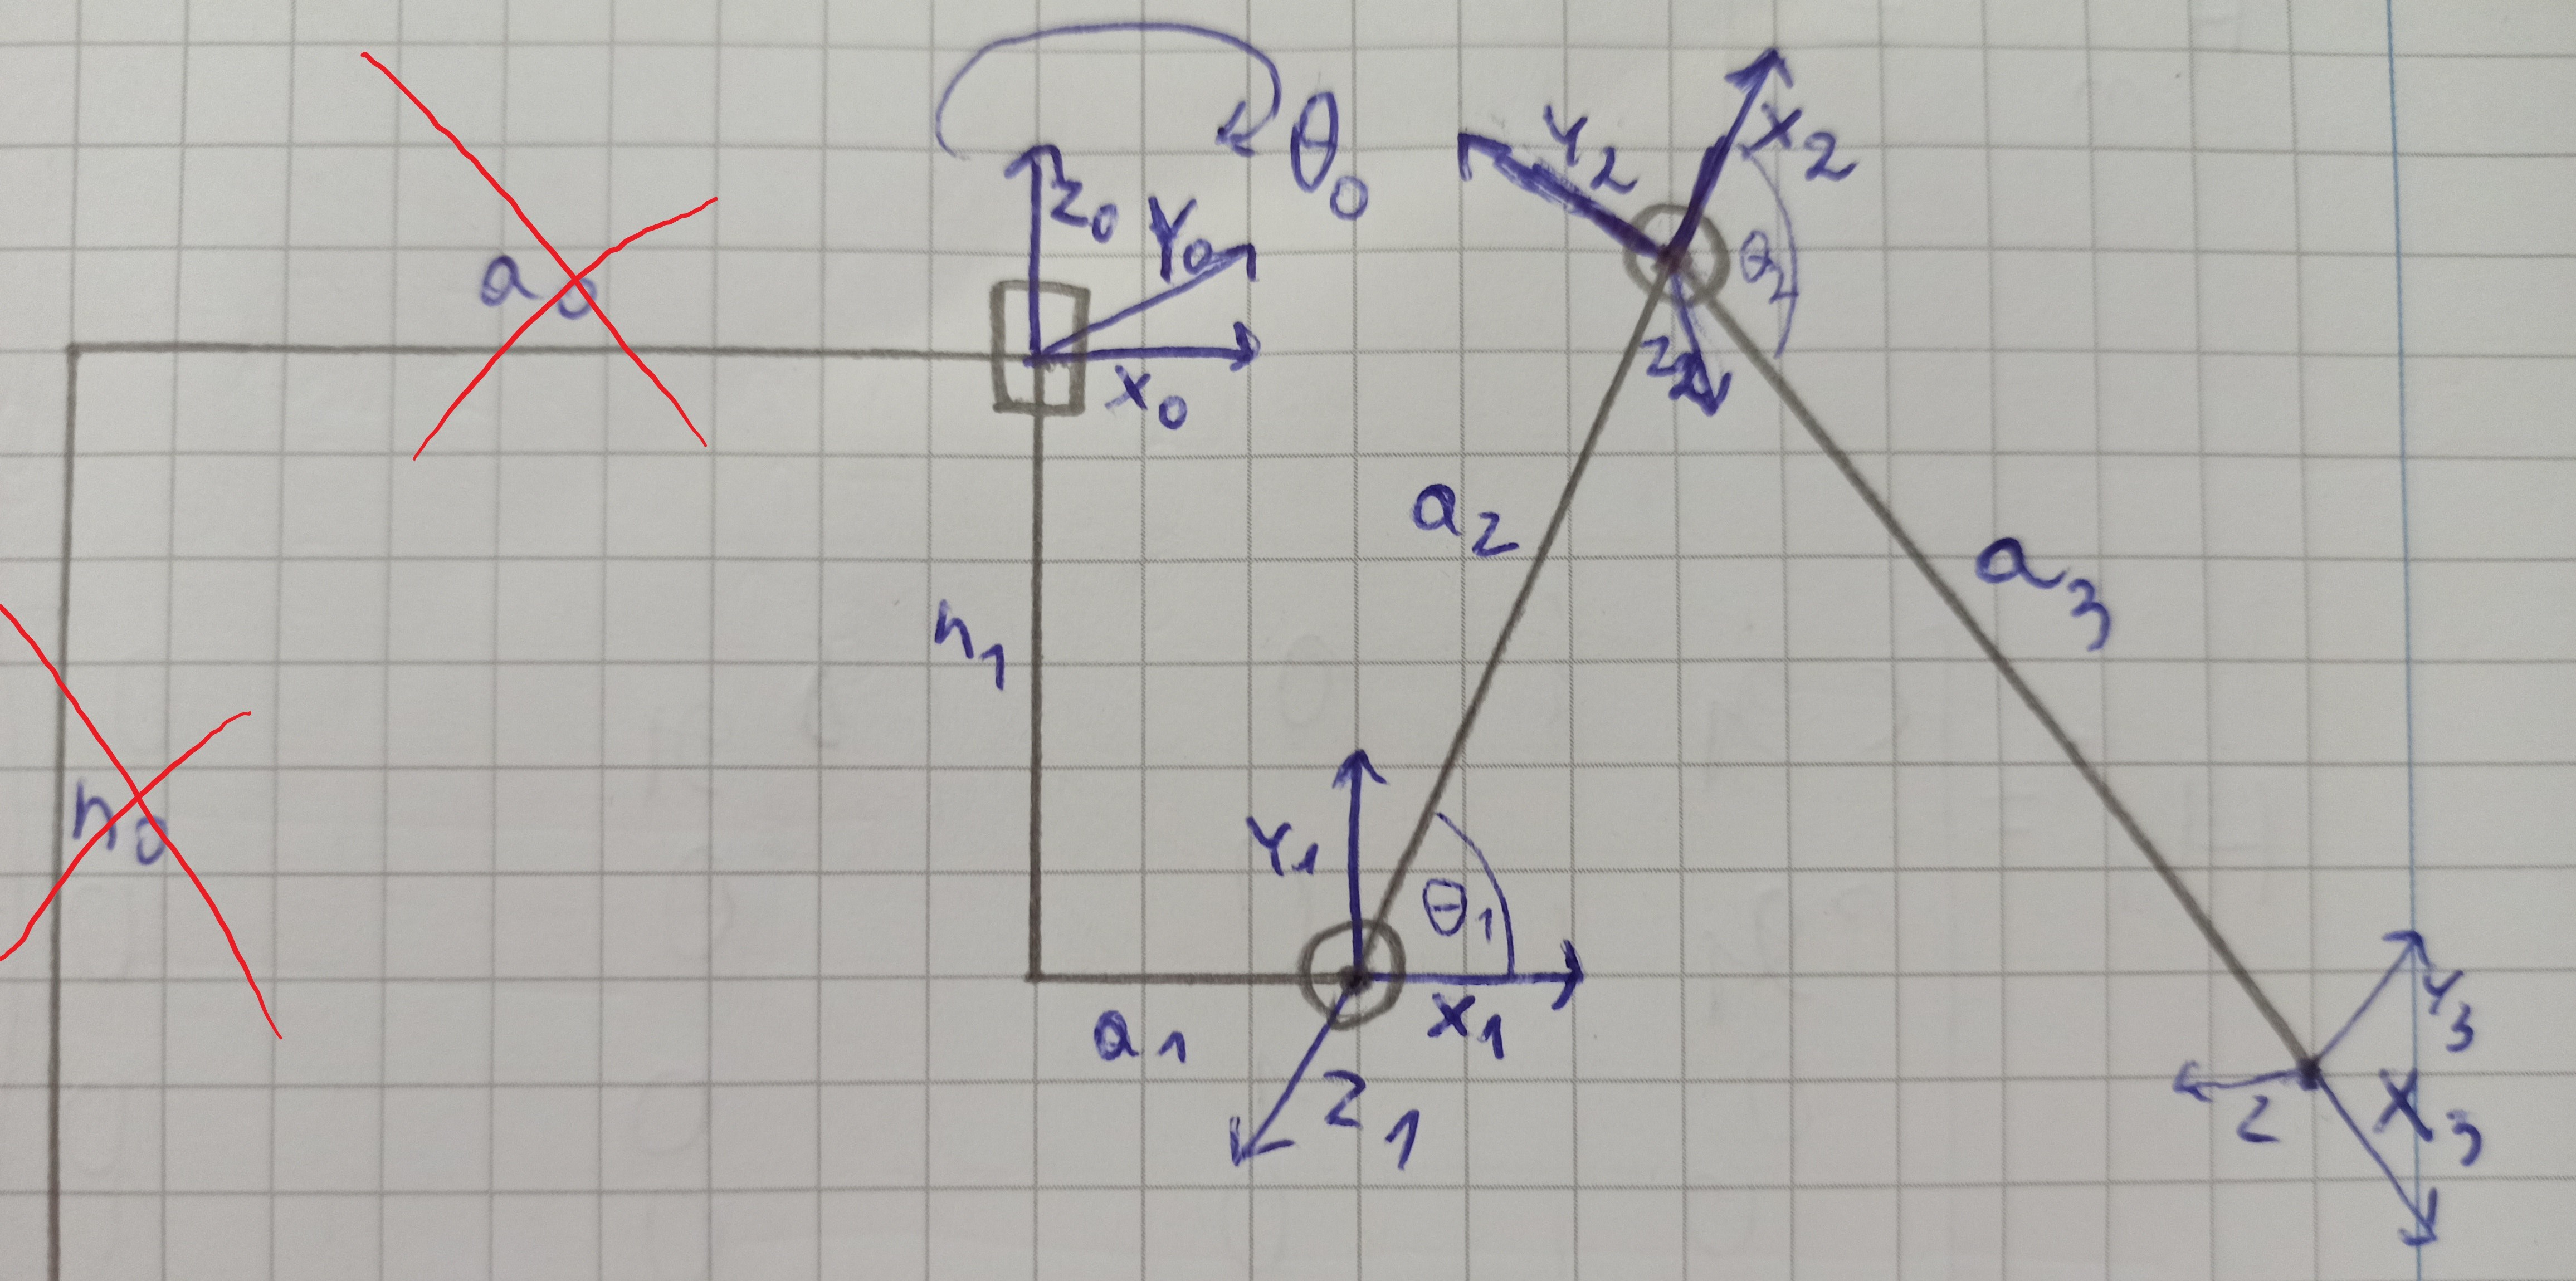
\includegraphics[width=\textwidth]{img/DH_model.jpg}
\caption{Model Denavit Hartenberg}
\label{math_model}
\end{figure}

\begin{equation}
\begin{array}{c|cccc}
\textrm{Joint } i & \theta_i & \alpha_i & r_i & d_i \\
\hline
1  & \theta_0 & \frac{\pi}{2} & a_1 & h_1 \\
2  & \theta_1 & 0 & a_2 & 0 \\
3  & \theta_2 & 0 & a_3 & 0 \\
\end{array}
\end{equation}

Gdzie: \\
$\theta_i$ - angle from $x_{n-1}$ to $x_n$ around $z_{n-1}$\\
$\alpha_i$ - angle from $z_{n-1}$ to $z_n$ around $x_n$\\
$r_i$ - distance between the origin of the $n-1$ frame and the origin of the $n$ frame along the $x_n$ direction.\\ 
$d_i$ - distance from $x_{n-1}$ to $x_n$ along the $z_{n-1}$ direction\\

Następnie macierze przejść pomiędzy ramkami $n-1$ i $n$ oblicza się zgodnie z następującym wzorem:

\begin{equation}
H^{n-1}_n = 
\left[\begin{array}{ccc|c}
&&&\\
&&&\\
\multicolumn{3}{c|}{\smash{\raisebox{0.75\normalbaselineskip}{R}}} & \smash{\raisebox{0.75\normalbaselineskip}{T}}\\
\hline
0 & 0 & 0 & 1\\
\end{array}\right] = 
\left[\begin{matrix}
\cos{\theta_i} & -\sin{\theta_i} \cdot \cos{\alpha_i} & \sin{\theta_i} \cdot \sin{\alpha_i} & a_i \cdot \cos{\theta_i}\\
\sin{\theta_i} & \cos{\theta_i} \cdot \cos{\alpha_i} & -\cos{\theta_i} \cdot \sin{\alpha_i} & a_i \cdot \sin{\theta_i}\\
0 & \sin{\alpha_i} & \cos{\alpha_i} & d_i\\
0 & 0 & 0 & 1\\
\end{matrix}\right]\cite{DH_matrix_AA_article}
\end{equation}

Gdzie $R$ oznacza macierz Rotacji a $T$ macierz Transformacji.\\

A macierz przejścia pomiędzy ramką 0 a ramką 3 zgodnie z następującym wzorem:


\begin{multline} \label{DH_final_equation}
H^{n-1}_n = H^0_1 \cdot H^1_2 \cdot H^2_3 =\\
\left[\begin{matrix}
c\theta_0 \cdot \left( c\theta_1 \cdot c\theta_2 - s\theta_1 \cdot s\theta_2 \right) & -c\theta_0 \cdot \left( c\theta_1 \cdot s\theta_2 + s\theta_1 \cdot c\theta_2 \right) & s\theta_0 & c\theta_0 \cdot \left( a_1 + a_2 \cdot c\theta_1 + a_3  \cdot \left( c\theta_1 \cdot c\theta_2 - s\theta_1 \cdot s\theta_2 \right) \right)\\
s\theta_0 \cdot \left( c\theta_1 \cdot c\theta_2 - s\theta_1 \cdot s\theta_2 \right) & -s\theta_0 \cdot \left( c\theta_1 \cdot s\theta_2 + s\theta_1 \cdot c\theta_2 \right) & -c\theta_0 & s\theta_0 \cdot \left( a_1 + a_2 \cdot c\theta_1 + a_3  \cdot \left( c\theta_1 \cdot c\theta_2 - s\theta_1 \cdot s\theta_2 \right) \right)\\
c\theta_1 \cdot s\theta_2 + s\theta_1 \cdot c\theta_2 & c\theta_1 \cdot c\theta_2 - s\theta_1 \cdot s\theta_2 & 0 & h_1 + a_2 \cdot s\theta_1 + a_3 \cdot \left( c\theta_1 \cdot s\theta_2 + s\theta_1 \cdot c\theta_2 \right)\\
0 & 0 & 0 & 1\\
\end{matrix}\right] = \\
\left[\begin{matrix}
c\theta_0 \cdot c\left( \theta_1 + \theta_2 \right) & -c\theta_0 \cdot s\left( \theta_1 + \theta_2 \right) & s\theta_0 & c\theta_0 \cdot \left( a_1 + a_2 \cdot c\theta_1 + a_3  \cdot c\left( \theta_1 + \theta_2 \right) \right)\\
s\theta_0 \cdot c\left( \theta_1 + \theta_2 \right) & -s\theta_0 \cdot s\left( \theta_1 + \theta_2 \right) & -c\theta_0 & s\theta_0 \cdot \left( a_1 + a_2 \cdot c\theta_1 + a_3  \cdot c\left( \theta_1 + \theta_2 \right) \right)\\
c\theta_1 \cdot s\theta_2 + s\theta_1 \cdot c\theta_2 & c\left( \theta_1 + \theta_2 \right) & 0 & h_1 + a_2 \cdot s\theta_1 + a_3 \cdot s\left( \theta_1 + \theta_2 \right)\\
0 & 0 & 0 & 1\\
\end{matrix}\right]
\end{multline}


%\left[\begin{matrix}
%\cos{\theta_0} \cdot \cos{\theta_1} \cdot \cos{\theta_2} & -cos{\theta_0} \cdot \sin{\theta_1} \cdot \sin{\theta_2}  & \sin{\theta_0} & \cos{\theta_0} \cdot \left( a_2 \cdot \cos{\theta_1} + a_3 \cdot \cos{\theta_1} \cdot \cos{\theta_2}\right)\\
%\sin{\theta_0} \cdot \cos{\theta_1} \cdot \cos{\theta_2} & -sin{\theta_0} \cdot \sin{\theta_1} \cdot \sin{\theta_2}  & \cos{\theta_0} & \sin{\theta_0} \cdot \left( a_2 \cdot \cos{\theta_1} + a_3 \cdot \cos{\theta_1} \cdot \cos{\theta_2}\right)\\
%\sin(\theta_1) \cdot \sin(\theta_2) & \cos(\theta_1) \cdot \cos(\theta_2) & 0 & a_2 \cdot \sin(\theta_1) + a_3 \cdot \sin(\theta_1) \cdot \sin(\theta_2)\\
%0 & 0 & 0 & 1\\
%\end{matrix}\right]

Następnie, aby otrzymać właściwe równania, należy z równania \ref{DH_final_equation} wziąć część odpowiedzialną za transformację.

\begin{equation}
\begin{split}
X &= c\theta_0 \cdot \left( a_1 + a_2 \cdot c\theta_1 + a_3  \cdot c\left( \theta_1 + \theta_2 \right) \right)\\
Y &= s\theta_0 \cdot \left( a_1 + a_2 \cdot c\theta_1 + a_3  \cdot c\left( \theta_1 + \theta_2 \right) \right)\\
Z &= h_1 + a_2 \cdot s\theta_1 + a_3 \cdot s\left( \theta_1 + \theta_2 \right)\\
\end{split}
\end{equation}



\subsubsection{Invert kinematics}
Odwrotną kinematykę można obliczyć poprzez rozwiązanie równań kinematyki prostej.

Najprościej jest wyprowadzić wzór na $\theta_0$, można to zrobić na podstawie wzoru \ref{FK_ver_1}, łącząc wzór na $X$ i $Y$:
\begin{equation}
\begin{split}
\begin{cases}
Y = a_{temp} \cdot \sin{\theta_0}\\
X = a_{temp} \cdot \cos{\theta_0}
\end{cases}
\end{split}
\end{equation}

\begin{equation}
\begin{split}
\begin{cases}
Y = a_{temp} \cdot \sin{\theta_0}\\
a_{temp} = \frac{X}{\cos{\theta_0}}
\end{cases}
\end{split}
\end{equation}


\begin{equation}
Y = \frac{X}{\cos{\theta_0}} \cdot \sin{\theta_0}\\
\end{equation}

\begin{equation}
\theta_0 = \arctan{\frac{Y}{X}}
\end{equation}

%Wzór na $\theta_2$ można wyprowadzić także z równania \ref{FK_ver_1}

%\[
%Z = (- h_1) + a_2 \cdot \sin{\theta_1} - a_3 \sin{\left( \theta_2 - \theta_1 %\right)}
%\]

%\[
%Z - h_1 = a_2 \cdot \sin{\theta_1} - a_3 \sin{\left( \theta_2 - \theta_1 \right)}
%\]

%\[
%\frac{h_1 - Z - a_2 \cdot \sin{\theta_1}}{a_3} = \sin{\left( \theta_2 - \theta_1 \right)}
%\]


%\begin{equation} \label{theta_2_eq}
%\theta_2 = \arcsin{\left(\frac{h_1 - Z - a_2 \cdot \sin{\theta_1}}{a_3}\right)} + \theta_1
%\end{equation}

%Równanie \ref{theta_2_eq} jest nadal uzależnione od $\theta_1$, które należy wyznaczyć.

N%ajbardziej oczywistym wydaje się pod równanie \ref{FK_ver_1} na $a_{temp}$ podstawić obliczone równanie \ref{theta_2_eq} i daje to równanie  \ref{theta_1_eq1}

%\begin{equation} \label{theta_1_eq1}
%a_{temp} = a_2 \cos{\theta_1} + a_3 \cos{\left(\arcsin{\left(\frac{h_1 - Z - a_2 \cdot \sin{\theta_1}}{a_3}\right)}\right)} + a_1\\
%\end{equation}

%Do fragmentu $a_3 \cos{\left(\arcsin{\left(\frac{h_1 - Z - a_2 \cdot \sin{\theta_1}}{a_3}\right)}\right)}$ można zastosować wzór $\cos{\left(\arcsin{\left(x\right)}\right)} = \sqrt{1 - x^2}$. Daje to wzór \ref{theta_1_eq2}

%\begin{equation} \label{theta_1_eq2}
%a_{temp} = a_2 \cos{\theta_1} + \sqrt{a_3^2 - (a_2 \sin{\theta_1} - h_1 - Z)^2} + a_1\\
%\end{equation}

%Niestety wzór \ref{theta_1_eq2} nie pozwala jednoznacznie wyznaczyć jawnego $\theta_1$ i co za tym idzie nie da się tego wzoru jednoznacznie zaimplementować softwareowo, co jest niezbędne w dalszej części pracy. Można natomiast powrócić do rysunku \ref{math_model} i zastosować na trójkącie utworzonym z $a_2$ i $a_3$ twierdzenie cosinusów połączone z twierdzeniem pitagorasa.

Jeżeli wyznaczanie równań $\theta_1$ i $\theta_2$ sprowadzi się do problemu dwuwymiarowego, obliczenia stają się w zasadzie identyczne jak w przypadku obliczeń kinematyki odwrotnej dla robota typu SCARA, co było już robione wielokrotnie.\\

Aby obliczyć kąt $\theta_2$ można powrócić do rysunku \ref{math_model} i zastosować na trójkącie utworzonym z $a_2$ i $a_3$ twierdzenie cosinusów połączone z twierdzeniem pitagorasa.

\begin{equation}
(x - a_1)^2 + (z - h_1)^2 = a_2^2 + a_3^2 - 2 \cdot a_2 \cdot a_3 \cdot \cos{(180^o - \theta_2)}\\
\end{equation}

\begin{equation}
\theta_2 = 180 - \arccos{\left( \frac{(x - a_1)^2 + (z - h_1)^2 - a_2^2 - a_3^2}{2 a_2 a_3} \right)}\\ \cite{SCARA_model}
\end{equation}
Natomiast obliczenia dla $\theta_1$ TODO

\begin{equation}
\theta_1 = \arctan{\frac{z - h_1}{x - a_1}} - \arcsin{\left( \frac{L_2 \sin{\theta_2} }{ \sqrt{ (x - a_1)^2 + (z - h_1)^2}} \right)}\\ \cite{SCARA_model}
\end{equation} 

TODO - ograniczenia.

\subsection{Cały Robot}
Zwykle konstruując roboty wzorujemy się na zwierzętach występujących w naturze. W tym przypadku nie mamy jednak tego luksusu, dlatego na początek należy przyjąć jakieś najbardziej intuicyjne założenie. Dlatego też uznałem że najlepszym rozwiązaniem będzie rozmieścić nogi na jednej płaszczyźnie w równych odstępach - co $120\deg$.

W poprzednim podrozdziale przyjąłem osie układu relatywne do ułożenia początkowego nogi robota. Oznacza to że robot trójnożny będzie miał 3 niezależne osie $x$ i 3 niezależne osie $y$, tylko oś $z$ zgadza się między kolejnymi nogami. Idzie za tym konieczność stworzenia pewnej metody "obracania" wszystkich tych osi $x$ i $y$ do jednego zunifikowanego układu współżędnych. Pozwoli to obliczyć konematykę całego robota.

\subsubsection{Matematyka kroku}
Aby móc w prosty sposób napisać później algorytmy chodu i móc się skupić na kolejności przestawiania nóg przez robota, długości i wysokości kroku i innych tego typu aspektach, należy teraz dobrze ten krok sparametryzować. Na podstawie moich poprzednich doświadczeń z podobnymi projektami, uważam że najbardziej intuicyjne będzie sparametryzowanie kroku do:
\begin{itemize}
\item wartości kąta pomiędzy kierunkiem "do przodu" kroku a osią $x$ danej nogi
\item długości kroku
\item wysokości kroku
\end{itemize}



\section{Model CAD i druk 3D}

\section{Środowisko ROS}
\subsection{Schemat implementacji}

\section{Algorytm Chodu}

\begin{thebibliography}{9}
\bibitem{DH_AA_article}
\href{https://automaticaddison.com/how-to-find-denavit-hartenberg-parameter-tables/}{How to Find Denavit-Hartenberg Parameter Tables, blogpost by Automatic Addison}

\bibitem{DH_matrix_AA_article}
\href{https://automaticaddison.com/homogeneous-transformation-matrices-using-denavit-hartenberg/}{Homogeneous Transformation Matrices Using Denavit-Hartenberg, blogpost by Automatic Addison}

\bibitem{DH_Matlab_calc}
\href{./DH_calculations.m}{Matlab Denavit Hartenberg calculations}

\bibitem{SCARA_model}
\href{https://sj.umg.edu.pl/sites/default/files/ZN20.pdf}{Adam Labuda, Janusz Pomirski, Andrzej Rak (2009) Model manipulatora o dwóch stopniach swobody}


\bibitem{}
\href{https://www.diva-portal.org/smash/get/diva2:1462059/FULLTEXT01.pdf}{Alexander Wallen Kiessling, Niclas Maatta (2020) Anthropomorphic Robot Arm}

\end{thebibliography}
\end{document}